\section{Turbines}
A meanline and simplified approach for turbomachine design can produce qualitative information of great value to the designers and engineers in the first phase of development with small computational cost as drawback. For instance, specific trends about turbine performance and operation ease the definition of machine basic geometry (dimensions and shapes), with low usage of temporal and computational resources.

The first phase consists of a detailed analysis of main requirements of the project. The engine cycle analysis provides information as inlet conditions, pressure ratio, mass flow and rotation. These variables are good candidates to be part of the inlet vector of a \textbf{black box} scheme.

The following relation of previous work are intended to be studied in this part of the dissertation:
\begin{enumerate}
    \item \cite{Saravanamuttoo2017}
    \item ME-211 class notes
    \item \cite{Ovsyannikov1971}
    \item \cite{Belyaev1999}
    \item \cite{IgorGeorge2020}
    \item \cite{Schobeiri2018}
    \item \cite{Denton1993}
    \item \cite{Maia2019}
    \item \cite{Denton1998}
    \item \cite{Craig1970}
    \item \cite{Leach1983}
    \item \cite{Kadhim2018}
    \item \cite{DentonWallis1998}
    \item \cite{Lee2018}
    \item \cite{Noh2004}
    \item \cite{Ohlsson1962}
    \item \cite{Cho2008}
    \item \cite{Varma2012}
\end{enumerate}

\subsection{Loss Models}

\section{Optimization}
The procedure of problem formulation starts on creating a mathematical model of the optimal design problem, in order to solve it by an optimization algorithm.

According to \cite{Deb2012} about problem formulation, it is necessary to realize firstly the need of using an optimization in this specific problem. The author also illustrate that optimization algorithms are routinely used in aerospace design activities to minimize the overall weight, since every element or component adds to the overall weight of the aircraft or spacecraft. Thus, the first step of this problem formulation is already satisfied.

Then, the next step is to choose the important design variables associated with the turbine problem. As said before, these variables can be fluid inlet thermodynamics properties conditions, pressure ratio through turbine stage, mass flow and rotation, since they came from requirements of high order components after engine cycle analysis.

In addition, the formulation of optimal design problems involves other considerations, such as constraints, objective function, and variable bounds, as suggested by \cite{Deb2012}.

The figure \ref{fig:od_flowchart} shows a sumarizing flowchart about the procedure illustrated previously. Once declared and defined the optimal design problem, it is chosen the suitable optimization algorithm.

\begin{figure}[h]
    \centering
    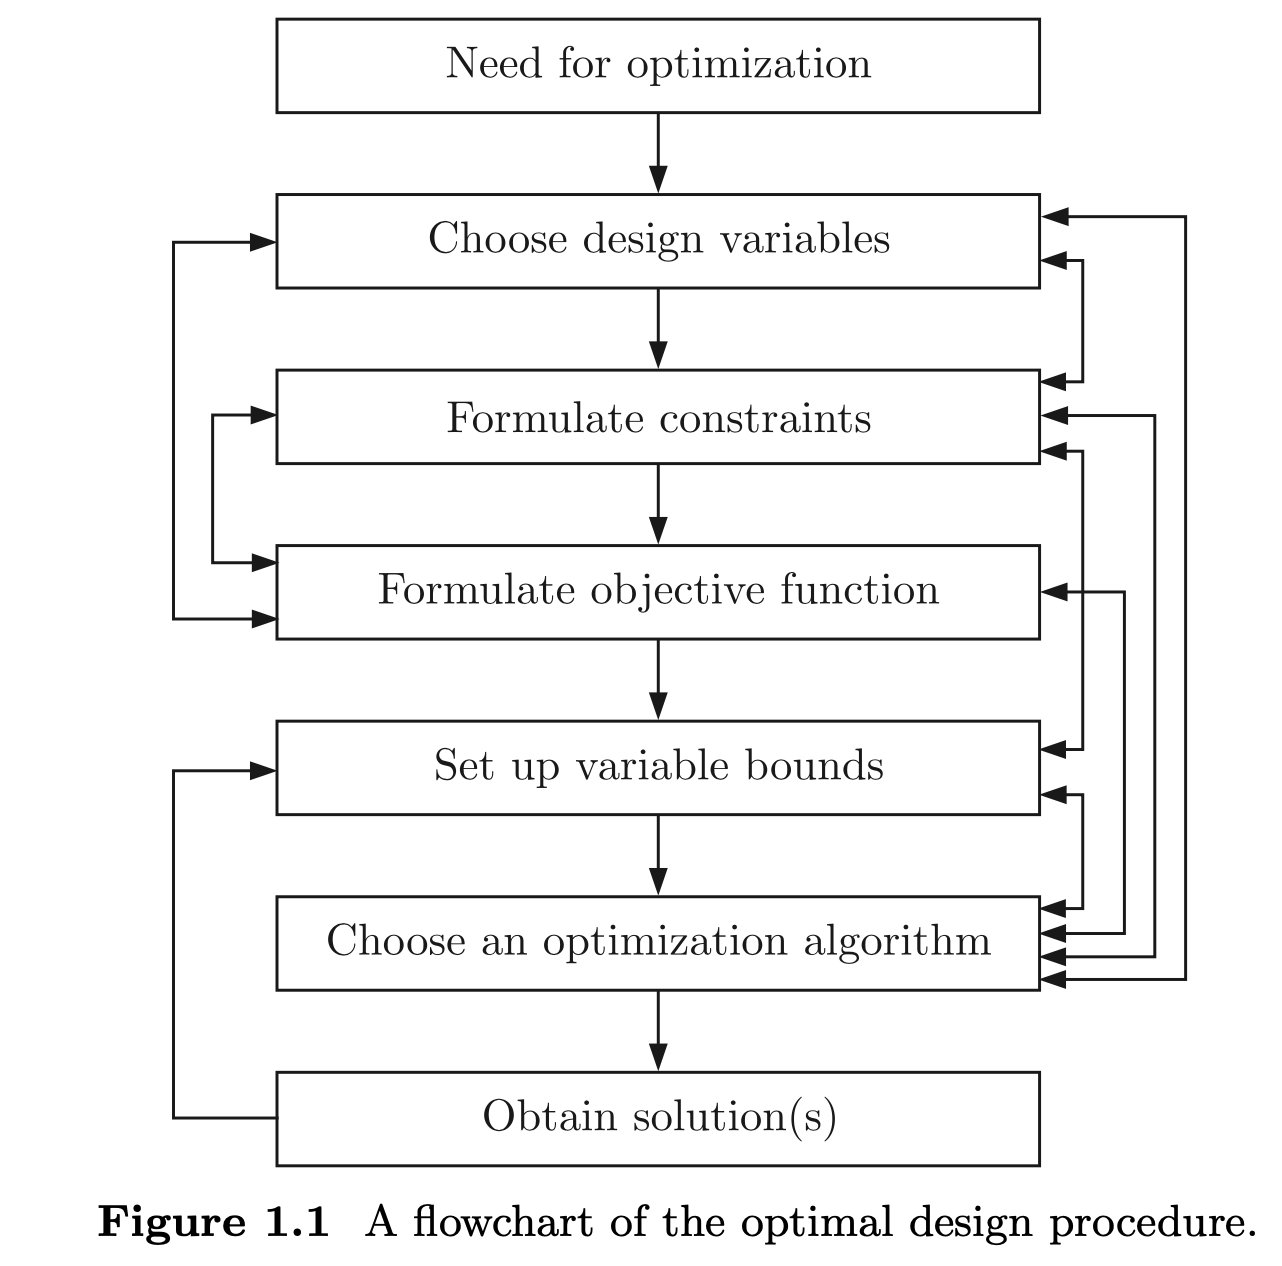
\includegraphics[width=0.75\textwidth]{Cap3/od_flowchart.png}
    \caption{Flowchart of the optimal design procedure. Source \cite{Deb2012}.}
    \label{fig:od_flowchart}
\end{figure}

\subsection{Root-Finding}
Finding the roots of an equation is common to many engineering activities and many root-finding problems are parts of the optimization process. This problem can be solved using an optimization technique by suitably choosing an objective function, as suggested by \cite{Deb2012}. The problem of finding $f(x)$ roots could be converted to, for instance, minimizing $\left|f(x)\right|$ or minimizing $\left[f(x)\right]^2$. The former has an advantage about using derivative-based optimization methods.

Once the optimization problem is formed, a bracketing technique can be used to first bracket the root and then a region-elimination method or a gradient-based search method can be used to find the root with the desired accuracy \cite{Deb2012}.

\subsection{Design Variables}
\subsubsection{Sensibility of design variables}
How impactant can be a variable in relation to an objective function. It is possible that a variable is more sensitive to an aspect than others.

\subsection{Objective Function}
It is suggested by \cite{Deb2012} the avoidance of several objective functions. Usually, it is selected the main of them and set it as unique objective function. Modification of the other functions comes along in order to force restrictions to the problem, bounding them into specific range, that was \textit{a priori} analised.

\subsection{Constraints}

\subsection{Design Variables Bounds}
It is set the bounds for design variables based on the previous analysis, and considering that the optimal solution is inside this range. Then, it is analised the firsts results and reset the interval for more precise results.

\subsection{Modeling}
Normally, mathematical modeling of the optimization problem is not easily reachable. An alternative is modify the governing equations, mainly when exist experimental and observed values of the system in study. Thus, if $E$ and/or any differential equations of $E$ describes a particular process, it is possible to add modification parameters and then a new equation as function of these parameters. The equation \ref{eq:reformulation} describes a possible function of search space $\beta$ (post-added parameters space), related to $E$ observed and simulated. Such process has similarities with a linear regression techniques, where $f$ represents the error or residue to be minimized.

\begin{equation}
f(\beta) = \left(E_{observed} - E_{simulated}\right)^2
\label{eq:reformulation}
\end{equation}

As demonstred by \cite{Deb2012}, the addition of these artificial parameters can bring advantages in the modeling and understanding of the problem, in terms of insights. 

The following relation of previous work are intended to be studied in this part of the dissertation:
\begin{enumerate}
    \item \cite{Mengistu2004}
    \item \cite{Asgarshamsi2014}
    \item \cite{Thorn2016}
    \item \cite{Arabnia2009}
    \item \cite{Cervantes2018}
    \item \cite{Juangphanich2019}
    \item \cite{Juangphanich2017}
    \item \cite{Agromayor2019}
    \item \cite{NooriRahimAbadi2017}
    \item \cite{Aminyavari2016}
    \item \cite{Ba2019}
    \item \cite{Lonard2008}
    \item \cite{ksz2010}
    \item \cite{Arabnia2012}
    \item \cite{Jenkins1982}
    \item \cite{Jenkins1983}
    \item \cite{Cervantes2018thesis}
    \item \cite{Sivashanmugam2011}
    \item \cite{Mengistu2005}
    \item \cite{Amano2003}
    \item \cite{Rao2012}
    \item \cite{Deb2012}
\end{enumerate}

\section{Problem Declaration}
The optimization task will be accomplished with the use of genetic algorithms, while the preliminary design of the turbine will be simplified and one-dimensional.

It is intended to use a simpler case study in order to understand the operation of the optimization and familiarization with the method. Such a base example can be done considering only one design variable. After this phase, the process formulated as a whole should be resolved. It is intended to limit the number of design variables to X, which are easily to make them dimensionless for comparison purposes.

\section{Genetic Algorithms}
According to \cite{Deb2012}, genetic algorithms allow a easy way to find multiples optimal solutions simultaneously in a single simulation run. In the case of multiobjective optimization problems, a set of optimal solutions emerges known as Pareto Optimal Solutios or Pareto Frontier.

\subsection{NSGA-II}
The following relation of previous work are intended to be studied in this part of the dissertation:
\begin{enumerate}
    \item \cite{Deb2002}
\end{enumerate}